\ts\space is a material in the group of \acp{TMD}.
All \ac{TMD} appear in the general form MX\textsubscript{2} with M being a layer of transition-metal atoms such as molybdenum, tungsten or titanium which are sitting between two layers of species X from the group of chalcogens like sulfur or selenium.
This covalently bonded structure is called a \ac{TMD} monolayer.
\Ac{TMD} bulk material is made up of many monolayers stacked monolayers, bonded by van-der-Waals interaction.

The research part of my studies will focus on the \ac{TMD} \textit{1T}-\ts, the \textit{1T}-prefix is referring to the stacking order of the monolayers, that results in octahedrally coordinated titanium atoms.
From here on out it will simply be referred to as \ts.
Its crystal structure at room temperature and atmospheric pressure is depicted in figure~\ref{fig:crystal}\,a.
The unit cell contains one Ti atom and two Se atoms and the lattice vectors have lengths of $|\mathbf{a}|=|\mathbf{b}|=3.541$\,\AA\space and $\mathbf{c}=6.001$\,\AA\cite{patel1983}.
The material shows semi-metallic electronic characteristics\cite{bachrach1976}, with a hole pocket from the Se 4s band at the $\Gamma$ point of the \ac{BZ} and an electron pocket at the L point from the Ti 3d band\cite{zunger1978}.

\begin{figure}[!t]
	\begin{minipage}{0.5\columnwidth}
		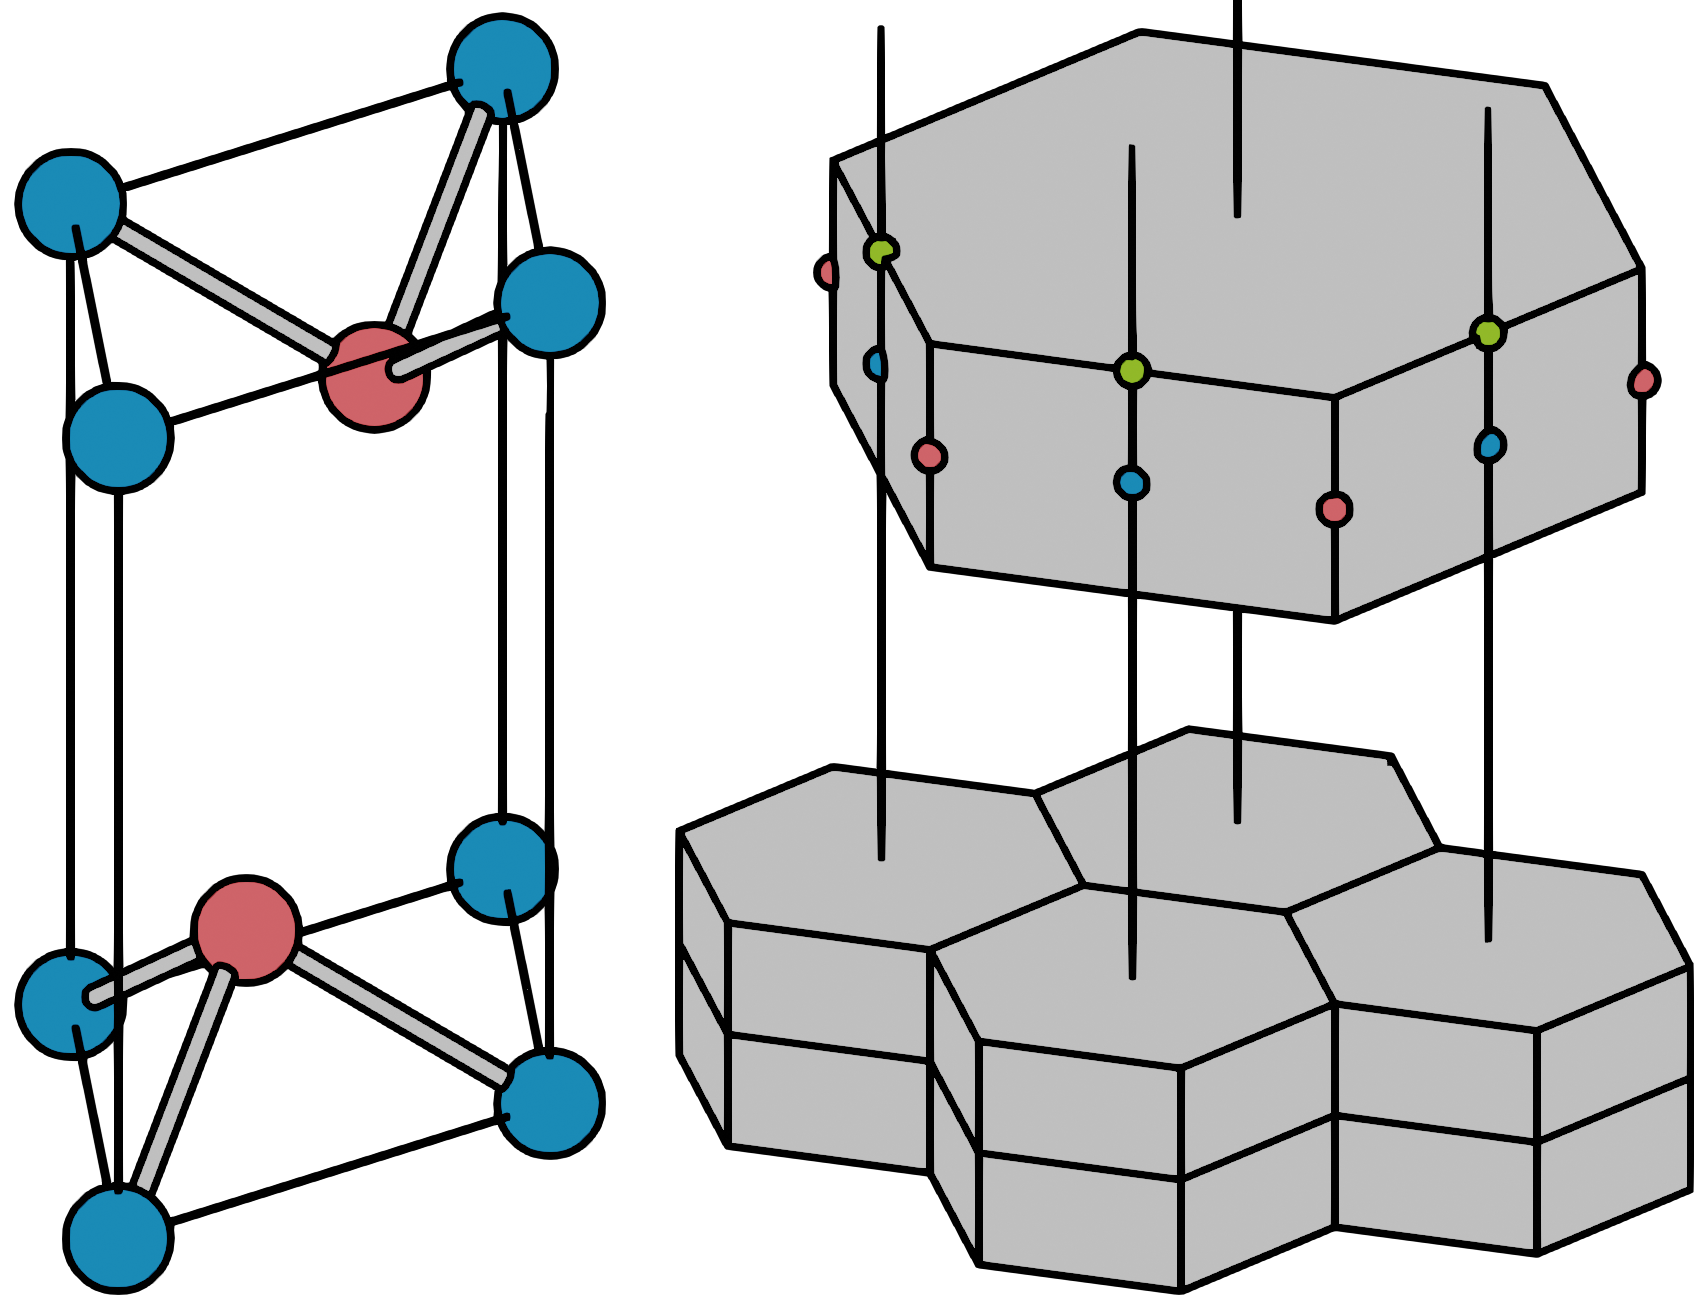
\includegraphics[width=\columnwidth]{figs/tise2_crystal.png}
	\end{minipage}
	\hspace{0.04\columnwidth}
	\begin{minipage}{0.45\columnwidth}
		\caption{\textbf{a)}\,Hexagonal unit cell of \ts, comprised of one Ti atom and two Se atoms. Ti atoms are shown in blue, Se atoms in red. \textbf{b)}\,\ac{BZ} of the high temperature phase (top) and low temperature phase (bottom) of \ts. Blue/red spheres mark M/L points in the \ac{BZ}}
		\label{fig:crystal}
	\end{minipage}
\end{figure}

Upon cooling, at 200\,K \cite{disalvo1976} \ts\space undergoes a second order phase transition into a phase with a commensurate $2\times2\times2$ \ac{PLD} accompanied by a \ac{CDW}\cite{rossnagel2011}.
The maximum displacement of the atoms is $u_\mathrm{max}/|\mathbf{a}|=2.4\%$\cite{disalvo1976}.
\ac{CDW} and \ac{PLD} go hand in hand, since a periodic modulation of the electron density will shift the equilibrium positions of the ions.
Vice versa, periodically displaced ions will alter the electron density to more adequately screen their potential.
Currently two mechanisms are discussed to drive the \ac{CDW}/\ac{PLD}: 
Firstly, the band Jahn-Teller effect describing the splitting of two degenerate energy bands due broken symmetry introduced by electron-phonon coupling and electron-lattice interaction\cite{JT}.
Secondly, the formation of a excitonic insulator ground state due to cooperative interaction between the charge carriers\cite{EI}.

Theoritical work shows that a \ac{CDW} phase transition driven by the band Jahn-Teller mechanism will be stable in materials with large electron-phonon coupling constants and large electronic susceptibilities\cite{friend1979}.
An alteration of the electron and phonon dispersion in form of a band gap opening at the fermi surface and a Kohn anomaly are predicted.
A Kohn anomaly will manifest itself as a strong phonon renormalization towads $\omega=0$\cite{kohn1959} (in this case at the M and L points in the \ac{BZ}).
This was previously observed with the very instrument that will be the key part of the proposed research\cite{otto2021}.
A phonon with vanishing frequency is often referred to as \emph{frozen} and corresponds to a static \ac{PLD} that does not require energy to form.
Density functional theory (DFT)\acused{DFT} simulations show that the superposition of the three freezing phonon modes at the M points are in good agreement with the experimentally observed \ac{PLD}\cite{kaneko2018}. % if first use is \AC, this thing fails...
The strong electron-phonon coupling in \ts\space results in a large lattice distortion, a large energy gap and a small coherence length of the \ac{CDW} phase\cite{haas1978,hildebrand2016}.

\begin{figure}[!t]
	\begin{minipage}{0.5\columnwidth}
		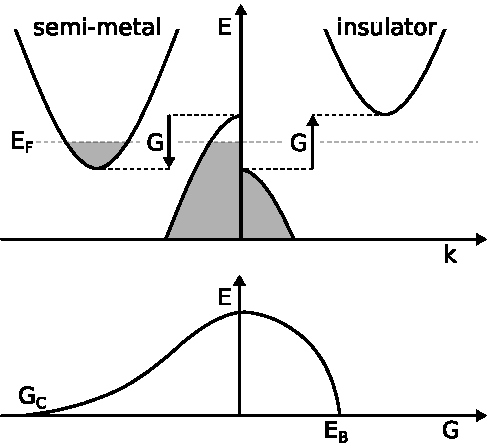
\includegraphics[width=\columnwidth]{figs/excitonic_insulator.pdf}
	\end{minipage}
	\hspace{0.04\columnwidth}
	\begin{minipage}{0.45\columnwidth}
		\caption{Band structure of a indirect semi-metal (\textbf{a}) with a band overlap of $G<0$ and an indirect insulator (\textbf{b}) with an indirect band gap of $G>0$ \textbf{c)} Net energy gain of the new excitonic ground state, between a critical band overlap $G_\mathrm{C}$ and a band gap up to the lowest exciton binding energy $E_\mathrm{B}$}
		\label{fig:ei}
	\end{minipage}
\end{figure}

A lower energy ground state created by charge carrier interaction is the so called excitonic insulator state, described by Kohn et al. in \cite{jerome1967, kohn1967}.
Considerring a semi-metal with a small indirect band overlap or a semiconductor with a small indirect band gap as shown in figure~\ref{fig:ei}\,a+b).
The small band overlap semi-metal can be seen as an insulator with few charge carriers.
Carriers are poorly screened and holes and electrons are attracting each other through Coulomb interaction, leading to exciton formation.
Exciton formation becomes more energetically favorable for smaller band overlaps starting at a critical overlap of $G_\mathrm{C}$, as shown in figure~\ref{fig:ei}\,c).
Starting from a normal insulator with band gap $G$ and reducing it, the system will at some point reach a state where the size of the band gap is the same as the energy of the lowest-lying exciton, $G-E_\mathrm{B}=0$.
This electronic instability leads to exciton formation, similar to the semi-metallic case.
Thus for $G_\mathrm{C}<G<E_\mathrm{B}$ the excitonic insulator ground state is stable.

Experimentally it is hard to distinguish both mechanisms.
However, analogous to the phonon softening in the band Jahn-Teller state, there will be a soft plasmon in the excitonic insulator state \cite{kohn1967, rossnagel2011}, this has been experimentally confirmed by momentum-resolved electron energy-loss spectroscopy\cite{kogar2017}.
The redistribution of charges inside the material will lead to \ac{CDW} formation, which can produce a \ac{PLD}.

Altough both approaches that have been discussed lead to qualitatively the same \ac{CDW}/\ac{PLD} phase, the underlying mechanisms are quite different.
The latter being driven by electron-electron and electron-hole interaction, whereas the former is mainly driven by strong electron-phonon coupling.

%misc
% describe difference in CDW/PLD from TiSe2 and other materials
% inverse width of kohn annomaly is measure for the coherence length